\documentclass{ximera}

\input{../../preamble.tex}
\author{Bobby Ramsey}

\begin{document}
\begin{exercise}
	The image below is the graph of which of the following functions?
	\begin{center}
		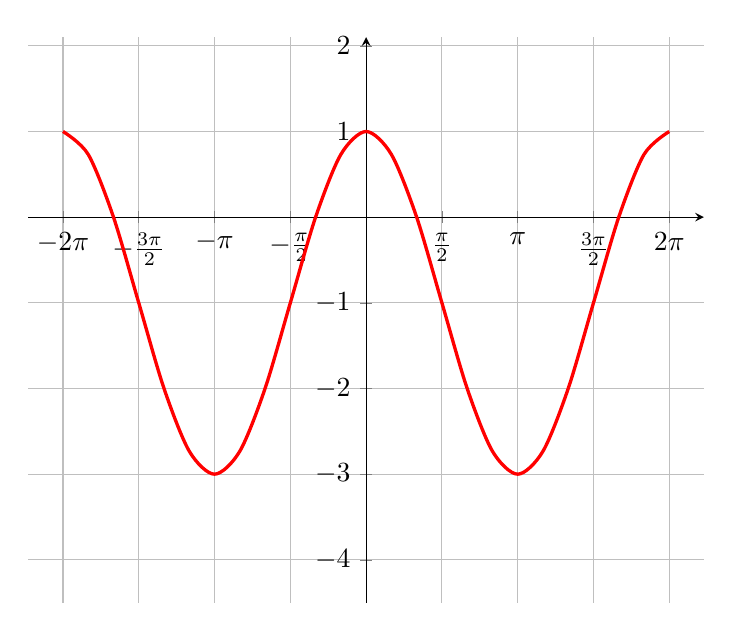
\begin{tikzpicture}
			\begin{axis}[
				xmin=-7, xmax=7, ymin=-4.5,ymax=2.1,    
				axis lines =middle, 
				every axis y label/.style={at=(current axis.above origin),anchor=south},
				every axis x label/.style={at=(current axis.right of origin),anchor=west},
				xtick={ -6.28318, -4.7123889, -3.14159, -1.5708,
        			1.5708, 3.14159, 4.7123889, 6.28318 },
    			xticklabels={ $-2\pi$, $-\frac{3\pi}{2}$, $-\pi$, 
    				$-\frac{\pi}{2}$, $\frac{\pi}{2}$, $\pi$, 
    				$\frac{3\pi}{2}$, $2\pi$}, 
    			ytick={-4,...,2},
				grid=major, width=4in,
				]
				\addplot[color=red, very thick, smooth, domain=-6.283:6.283]{ -1+2*cos(deg(x)) };
			\end{axis}
		\end{tikzpicture}
	\end{center}
	
	Select any/all correct answer/answers.
	\begin{selectAll}
		\choice[correct]{$2\cos(x)-1$}
		\choice{$2\sin(x)-1$}
		\choice{$-2\cos\left( x - \frac{\pi}{2} \right) - 1$}
		\choice[correct]{$-2\sin\left( x - \frac{\pi}{2} \right) - 1$}
		\choice{None of the above.}
	\end{selectAll}
\end{exercise}

\end{document}

